\documentclass[border=5pt]{standalone}
\usepackage[utf8]{inputenc}
\usepackage{amssymb}
\usepackage{amsmath}
\usepackage{tikz}
\usetikzlibrary{arrows.meta}

\begin{document}
\nopagecolor
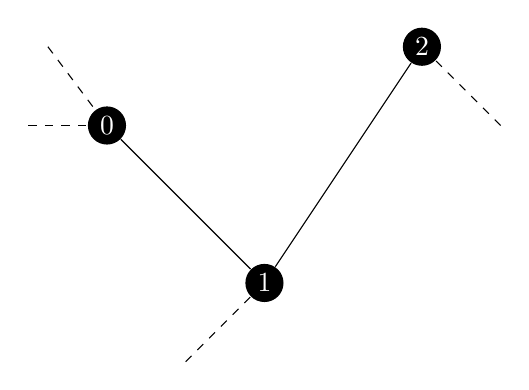
\begin{tikzpicture}
    \node[circle, inner sep=2pt, fill] (0) at (0, 0) {\color{white} 0};
    \node[circle, inner sep=2pt, fill] (1) at (2, -2) {\color{white} 1};
    \node[circle, inner sep=2pt, fill] (2) at (4, 1) {\color{white} 2};
    
    \draw (0) edge (1)
          (1) edge (2);
    \draw[dashed] (-1, 0) edge (0);
    \draw[dashed] (-0.75, 1) edge (0);
    \draw[dashed] (1, -3) edge (1);
    \draw[dashed] (5, 0) edge (2);
\end{tikzpicture}
\end{document}